\chapter{Equipment}
\label{chap:equip}


\section{Sidearms}
\label{sec:sidearms}

\subsection{b3 Wingman}

\begin{wrapfigure}[4]{l}{.34\linewidth}
\vspace*{-2em}
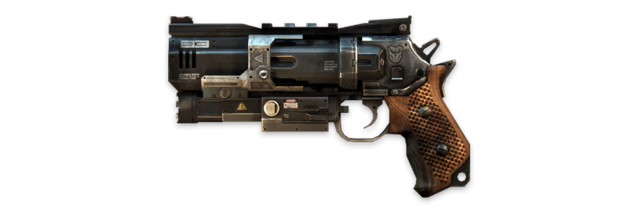
\includegraphics[width=\linewidth]{B3wingman}
\end{wrapfigure}

The B3 Wingman is an extremely powerful revolver with very high accuracy out to long ranges. Precision aim is required to mitigate the disadvantages of its very low rate of fire. 

\subsection{Hammond P2011}

\begin{wrapfigure}[4]{r}{.34\linewidth}
\vspace*{-2em}
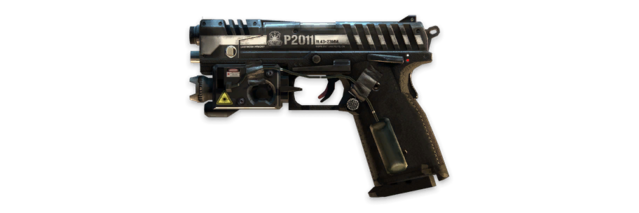
\includegraphics[width=\linewidth]{HammondP2011}
\end{wrapfigure}

The Hammond P2011 is a semi-automatic handgun with good accuracy and damage at range. Its integrated 'match trigger' allows it to be fired very rapidly, which is useful in close quarters. 

\subsection{RE-45 Autopistol}

\begin{wrapfigure}[3]{l}{.34\linewidth}
\vspace*{-2em}

\includegraphics[width=\linewidth]{RE45Autopistol}
\end{wrapfigure}


The RE-45 is a fully automatic .45 caliber pistol, sacrificing damage and accuracy at longer distances for improved effectiveness at close range.

\subsection{Smart Pistol mkv}

\begin{wrapfigure}[7]{r}{.34\linewidth}
\vspace*{-2em}
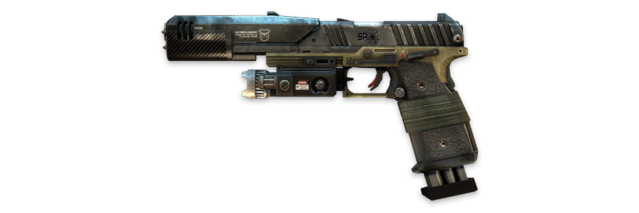
\includegraphics[width=\linewidth]{SmartPistolMK5}
\end{wrapfigure}

The Smart Pistol scans for hostile targets within a short range, locking onto them automatically. Any rounds fired will then maneuver to hit the locked targets. Aiming with the iron sights allows the operator to use the pistol in manual targeting mode. Due to the low magazine capacity, however, this weapon can run out of ammo by spending \Threat\Threat\Threat\ (instead of the normal \Despair). Spare ammunition for the smart pistol is twice the price as normal ammo, 50 credits.

\begin{table}[h!]
\caption{Sidearms}
\footnotesize
\begin{GenesysTable}{*{2}{l} *{2}{c} l c c r c X[l]}
Name & Skill & Dam & Crit & Range & Enc & HP & Price & Rarity & Special\\
B3 Wingman & Ranged (Light) & 6 & 3 & Medium & 1 & 1 & 500 & 3 & \\
Hammond P2011 & Ranged (Light) & 5 & 4 & Medium & 1 & 1 & 150 & 3 & \\
RE-45 Autopistol & Ranged (Light) & 5 & 3 & Short & 2 & 1& 300 & 6 & Accurate 1 \\
Smart pistol mk5 & Ranged (Light) & 5 &  3 & Short & 1 & 1 & 450 & 8 & Guided 3, Special\\

\end{GenesysTable}
\end{table}


\pagebreak
\section{Longarms}
\label{sec:rifles}

\subsection{R101C Carbine}
\begin{wrapfigure}[2]{l}{.34\linewidth}
\vspace*{-2em}
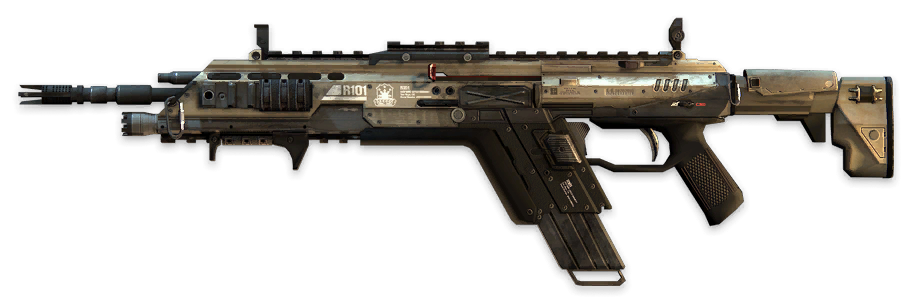
\includegraphics[width=\linewidth]{R101CCarbine}
\end{wrapfigure}


The R-101C is a fully automatic, compact assault weapon commonly used throughout the Frontier. 


\subsection{Hemlock BF-R}
\begin{wrapfigure}[5]{r}{.36\linewidth}
\vspace*{-2em}
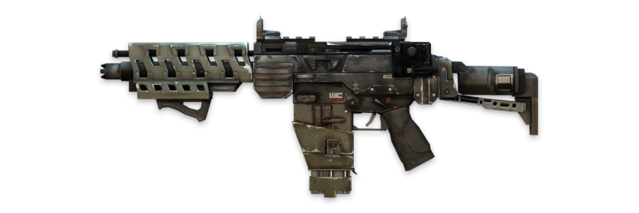
\includegraphics[width=\linewidth]{HemlokBFR}
\end{wrapfigure}
The factory issue Hemlok fires a three-round burst. While this can be a liability at short range, this tradeoff allowed the engineers at TW Ordnance to deliver a weapon with a good balance of long-range accuracy, damage, and fire rate.

\subsection{G2A4 Battle Rifle}
\begin{wrapfigure}[4]{l}{.36\linewidth}
\vspace*{-2em}
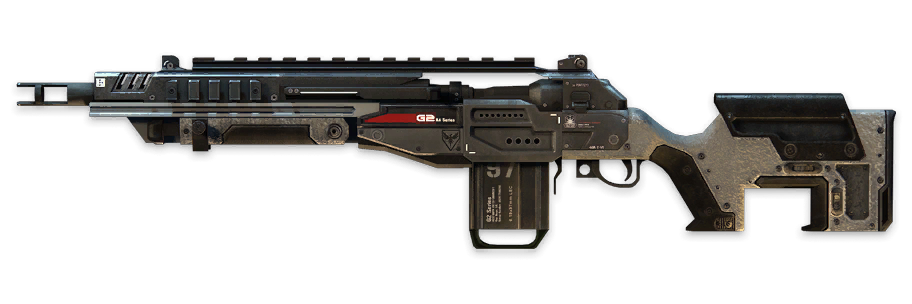
\includegraphics[width=\linewidth]{G2A4Rifle}
\end{wrapfigure}


Despite recent advances in weapons technology, the older G2A4 semi-automatic rifle remains a favorite of special forces units due to its high damage and extremely precise fire---a testament to its high level of craftsmanship.

\subsection{EVA-8 Shotgun}
\begin{wrapfigure}[5]{r}{.36\linewidth}
\vspace*{-2em}
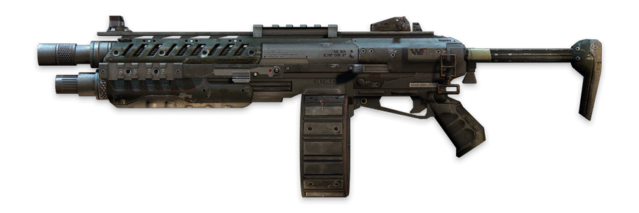
\includegraphics[width=\linewidth]{EVA8Shotgun}
\end{wrapfigure}


The EVA-8 is a semi-automatic shotgun, originally designed for extra-vehicular activity, both in conventional and in exo-atmospheric conditions. The low capacity and quick trigger means that the EVA-8 can run out of ammo by spending \Threat\Threat\Threat\ (instead of the normal \Despair).

\subsection{R-97 Compact SMG}
\begin{wrapfigure}[3]{l}{.36\linewidth}
\vspace*{-2em}
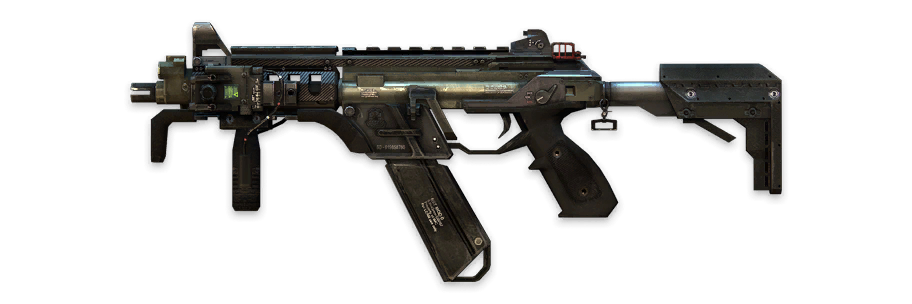
\includegraphics[width=\linewidth]{R97CompactSMG}
\end{wrapfigure}

The R-97 is a compact submachine gun that excels at close-quarters combat, due to its extremely high rate of fire and minimal recoil.

\subsection{C.A.R. SMG}
\begin{wrapfigure}[4]{r}{.36\linewidth}
\vspace*{-2em}
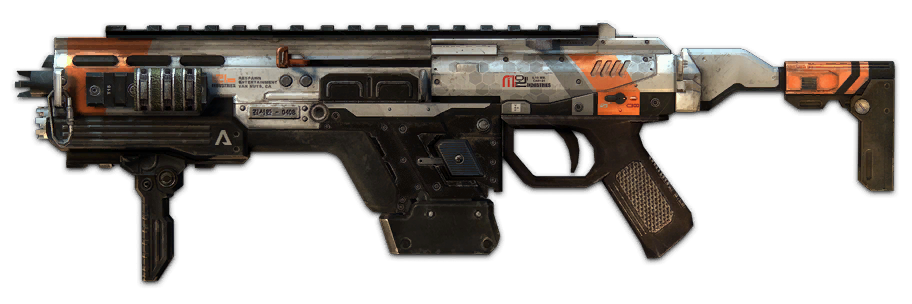
\includegraphics[width=\linewidth]{CARSMG}
\end{wrapfigure}

The C.A.R. (Combat Advanced Round) submachine gun is designed to fire a more powerful round that provides greater damage and accuracy at range, at the cost of fire rate and capacity.


\subsection{D-101 Longbow DMR}
\begin{wrapfigure}[3]{l}{.36\linewidth}
\vspace*{-2em}
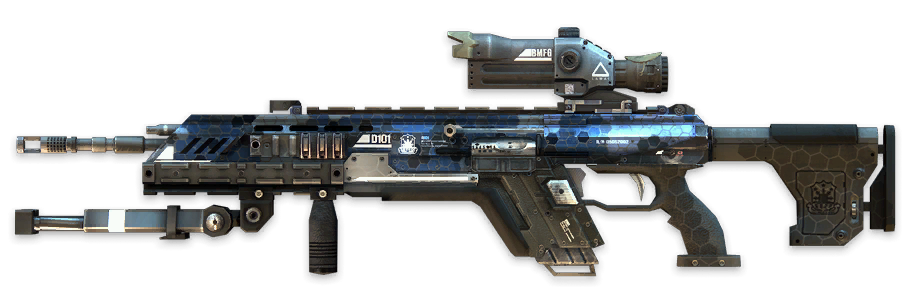
\includegraphics[width=\linewidth]{LongbowDMRSniper}
\end{wrapfigure}

The Longbow-DMR is a semi-automatic sniper rifle. Its hyper-velocity round completely eliminates the need to lead targets, and allows the shooter to fire multiple shots quickly in succession.


\subsection{Kraber-AP Sniper}
\begin{wrapfigure}[4]{r}{.36\linewidth}
\vspace*{-2em}
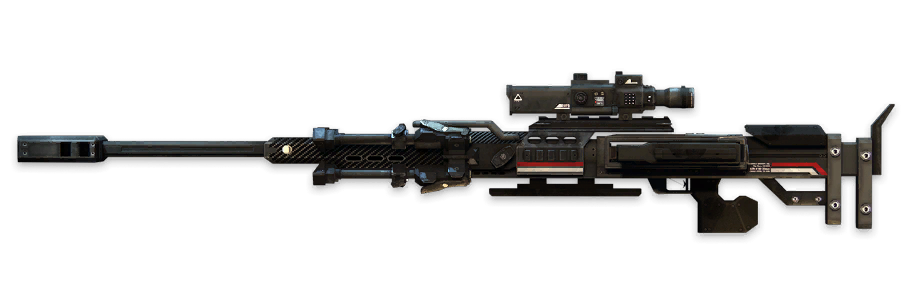
\includegraphics[width=\linewidth]{KraberAPSniper}
\end{wrapfigure}

The Kraber fires a unique round that ensures 'one-shot, one-kill' results against human-scale targets. However, considerable judgement in leading is required, making this a difficult weapon to use against moving targets.

\subsection{Spitfire LMG}
\begin{wrapfigure}[4]{l}{.36\linewidth}
\vspace*{-2em}
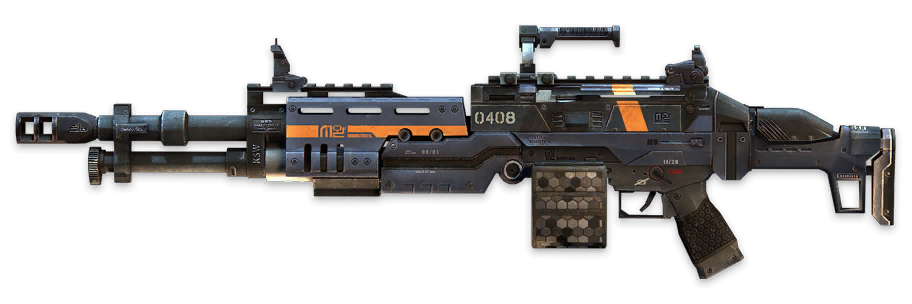
\includegraphics[width=\linewidth]{SpitfireLMG}
\end{wrapfigure}

The Spitfire Light Machine Gun recoils heavily when first fired, but quickly settles into a tight firing pattern. The manufacturer strongly recommends sustained saturating fire, instead of short controlled bursts.


\begin{table}[h!]
\caption{Longarms}
\footnotesize
\begin{GenesysTable}{*{2}{l} *{2}{c} l c c r c X[l]}
Name & Skill & Dam & Crit & Range & Enc & HP & Price & Rarity & Special\\
R-101C Carbine & Ranged (Heavy) & 8 & 3 & Long & 4 & 2 & 1,050 & 7 & Auto-fire\\
Hemlock BF-R & Ranged (Heavy) & 8 & 3 & Long & 4 & 2 & 1,000 & 7 & Accurate 1\\
G2A4 Battle Rifle & Ranged (Heavy) & 8 & 3 & Long & 4 & 2 & 950 & 6 &  \\ 
EV-8 Shotgun & Ranged (Heavy) & 8 & 3 & Short & 3 & 2 & 625 & 4 & \Special{Blast 6, Knockdown, Special}
R-97 SMG & Ranged (Heavy) & 6 & 3 & Medium & 3 & 2 & 750 & 6 & \Special{Auto-fire, Accurate 1}
C.A.R. SMG & Ranged (Heavy) & 7 & 3 & Medium & 3 & 2 & 550 & 6 & \Special{Accurate 2, Limited Ammo 2}
Longbow DMR & Ranged (Heavy) & 9 & 3 & Long & 4 & 2 & 1,000 & 5 & Accurate 1\\
Kraber & Ranged (Heavy) & 12 & 2 & Extreme & 5 & 3 & 2,000 & 8 & \Special{Accurate 2, Limited Ammo 1, Pierce 2}
Spitfire LMG & Gunnery &10 & 3 & Long & 6 & 3 & 1,750 & 6 & \Special{Auto-fire, Cumbersome 2, Pierce 2, Vicious 2}
\end{GenesysTable}
\end{table}

\section{Pilot Ordnance}
\label{sec:pilotordnance}

\subsection{Special Rules}
\textbf{Set Explosives.} The arc mine is an unusual ordnance in that you don't throw it at your opponent but rather set it in place and wait for someone to trigger the explosion. As an action you may set up to two mines within Engaged range of you. Then, when someone or something enters engaged range with the mine you make an Engineering combat check against the target.


\subsection{Arc Grenade}
\begin{wrapfigure}[4]{r}{.36\linewidth}
\vspace*{-2em}

\includegraphics[width=\linewidth]{ArcGrenade}
\end{wrapfigure}

The Arc Grenade is by infantry of the IMC and Militia. When activated, the Arc Grenade explodes in a blast of Arc energy capable of short circuiting and dealing heavy damage to robotic units and equipment such as Titans, Spectres, Stalkers, HUDs and optical equipment found within the helmet of a Pilot and Reapers. An arc grenade can negate Defense granted by energy shields by spending \Advantage\Advantage.

\subsection{Arc Mine}
\begin{wrapfigure}[6]{l}{.36\linewidth}
\vspace*{-2em}\centering
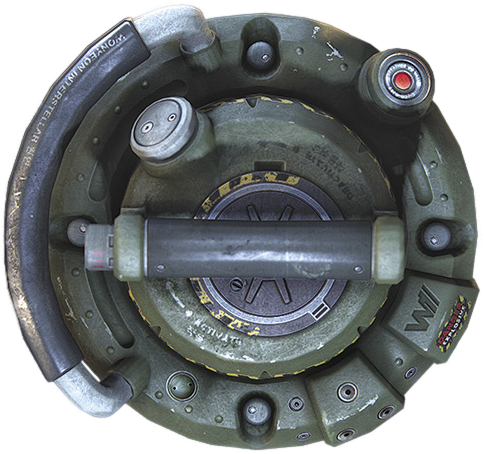
\includegraphics[width=0.5\linewidth]{ArcMine}
\end{wrapfigure}

The Arc Mine is a proximity mine that can stick on any surface. It takes 1 second after sticking to something to arm. Arc Mines won't explode until an enemy Pilot, Titan, Grunt, or Spectre enter the mine's range. An arc mine can negate Defense granted by energy shields by spending \Advantage\Advantage.

\subsection{Electric Smoke Grenade}
A pilot-portable version of the Titan defense system, this ``grenade" is designed to obscure an area and disperse pilots in an entrenched position. Any non-Titan target who stays within the cloud must make a \textbf{Hard (\DifficultyDie\DifficultyDie\DifficultyDie) Resilience check} at the end of their next turn or suffer 3 strain, plus 1 additional strain per \Failure. If the check generates \Threat\Threat, you may activate the Disorient quality.

The cloud creates two dice worth of concealment and completely blocks the Guided weapon quality on any attack against a target within the cloud or if the weapon must target through the cloud.

\subsection{Firestar}
The firestar is an incendiary throwing star that creates thermite on impact. It will stick to surfaces and enemies alike.


\subsection{Frag Grenade}
\begin{wrapfigure}[2]{r}{.36\linewidth}
\vspace*{-2em}

\includegraphics[width=\linewidth]{FragGrenade}
\end{wrapfigure}

The basic explosive device known to all modern soldiers, the Frag Grenade is still an incredibly useful weapon.

\subsection{Satchel Charge}
\begin{wrapfigure}[6]{l}{.36\linewidth}
\vspace*{-2em}
\centering
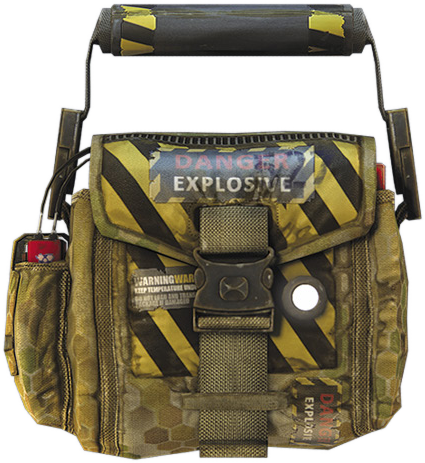
\includegraphics[width=.4\linewidth]{SatchelCharge}
\end{wrapfigure}

Satchel Charges stick to any surface and are manually detonated, causing massive explosive damage to anything nearby. Like mines, satchel charges are set and triggered to explode. Unlike a mine, however, you must trigger them yourself. As an action you may place up to two charges within Engaged range. As an out-of-turn incidental you may detonate the charges, making an Engineering combat check against the target.


\begin{table}[h!]
\caption{Ordnance}
\footnotesize
\begin{GenesysTable}{*{2}{l} *{2}{c} l c c r c X[l]}
Name & Skill & Dam & Crit & Range & Enc & HP & Price & Rarity & Special\\
Arc Grenade & Ranged (Light) & 5 & 4 & Short & 1 & 0 & 55 & 6 & \Special{Blast 4, Disorient 2, Limited Ammo 1, Stun Damage, Special}
Arc Mine & Mechanics & 6 & 4 & Engaged & 3 & 0 & 70 & 7 & \Special{Blast 5, Disorient 2, Limited Ammo 1, Stun Damage, Special}
Electric Smoke & Ranged (Light) & 4 & 6 & Short & 1 & 0 & 50 & 7 & \Special{Blast 3, Disorient 2, Limited Ammo 1, Stun Damage, Special}
Firestar & Ranged (Light) & 8 & 2 & Short & 1 & 0 & 100 & 7 & Burn 1, Limited Ammo 1\\
Frag Grenade & Ranged (Light) & 8 & 3 & Short & 1 & 0 & 90 & 7 & \Special{Blast 6, Limited Ammo 1}
Satchel Charge & Mechanics & 12 & 2 & Engaged & 2 & 0 & 280 & 6 & \Special{Blast 8, Breach 1, Limited Ammo 1, Special}
\end{GenesysTable}
\end{table}



\section{Anti-Titan Weapons}
\label{sec:antititanweapons}


\subsection{Archer Heavy Rocket}
\begin{wrapfigure}[4]{r}{.36\linewidth}
\vspace*{-2em}
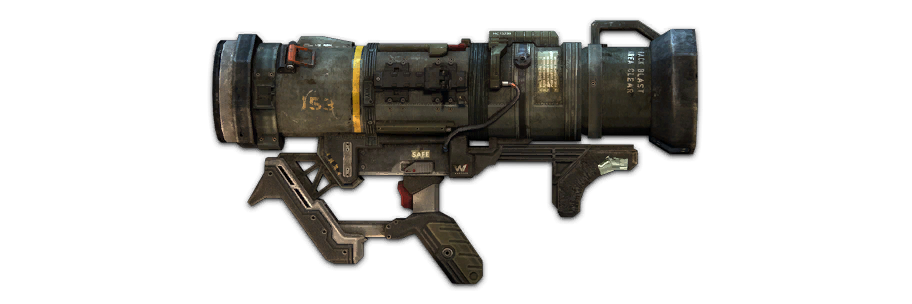
\includegraphics[width=\linewidth]{ArcherHeavyRocket}
\end{wrapfigure}

The Archer fires a powerful homing rocket. It must be locked onto a target before it can be fired. When aimed, a targeting window flips out, allowing target acquisition. Hold this window over the target continuously until a lock is achieved, then fire. The Guided quality can only be activated when attacking targets made of significant metal content, like Titans and Spectres. Reload rockets for the Archer cost 3,000 credit.

\subsection{Charge Rifle}
\begin{wrapfigure}[4]{l}{.36\linewidth}
\vspace*{-2em}
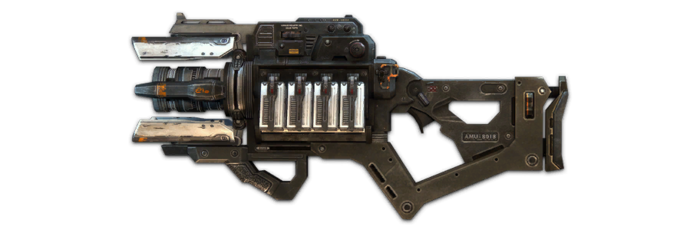
\includegraphics[width=\linewidth]{ChargeRifle}
\end{wrapfigure}

The Charge Rifle fires an energy beam that inflicts massive damage. Holding the trigger charges the weapon. Timing is critical to its use: this weapon will only fire when it reaches full charge, and it will discharge automatically as soon as it hits full charge.



\subsection{Mag Launcher}
\begin{wrapfigure}[3]{r}{.36\linewidth}
\vspace*{-2em}
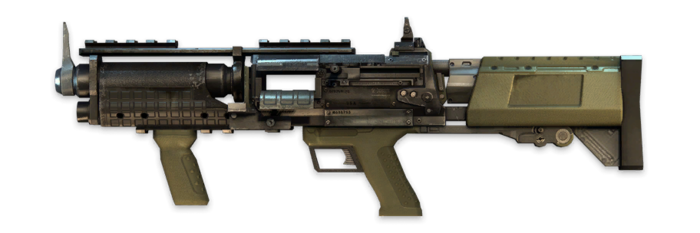
\includegraphics[width=\linewidth]{MagLauncher}
\end{wrapfigure}


The Mag Launcher fires magnetic grenades. When fired, the grenades will veer towards nearby enemy Titans and Spectres, and detonate on impact. The Guided quality can only be activated when attacking targets made of significant metal content, like Titans and Spectres. Due to the low magazine capacity, however, this weapon can run out of ammo by spending \Threat\Threat\Threat\ (instead of the normal \Despair).

\subsection{Sidewinder}
\begin{wrapfigure}[5]{l}{.36\linewidth}
\vspace*{-2em}
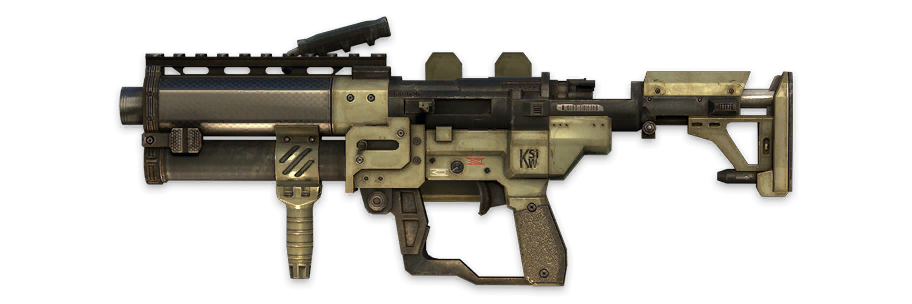
\includegraphics[width=\linewidth]{Sidewinder}
\end{wrapfigure}

The Sidewinder is a rapid-fire micro-missile launcher. It is effective against large targets, but lacks precision due to its large spread. The micro-missiles it fires do not yield a large area effect on detonation, due to their shaped-charge design.


\begin{table}[h!]
\caption{Anti-Titan Weapons}
\footnotesize
\begin{GenesysTable}{*{2}{l} *{2}{c} l c c r c X[l]}
Name & Skill & Dam & Crit & Range & Enc & HP & Price & Rarity & Special\\
Archer Rocket & Gunnery & 30 & 2 & Extreme & 8 & 4 & 10,525 & 8 & \Special{Blast 20, Breach 2, Cumbersome 3, Guided 3, Limited Ammo 1, Prepare 1}
Charge Rifle & Gunnery & 9 & 2 & Extreme & 8 & 4 & 3,250 & 7 & \Special{Accurate 1, Breach 2, Cumbersome 2, Slow-Firing 1, Vicious 2}
Mag Launcher & Gunnery & 12 & 3 & Long & 6 & 3 & 3,450 & 7 & \Special{Breach 2, Guided 2, Special}
Sidewinder & Gunnery & 18 & 2 & Medium & 6 & 3 & 5,075 & 6 & \Special{Auto-fire, Breach 2, Cumbersome 2, Inaccurate 1, Limited Ammo 3, Vicious 1}
\end{GenesysTable}
\end{table}

\section{Armour}

\subsection{Armoured Carapace}
Armoured carapace completely covers the wearer from head to toe and with the right attachments can be environmentally sealed. The carapace has a rigid outer shell that deflects or blocks incoming attacks. It is also designed to be extremely customizable, with one more hard point than a comparable size armour would otherwise have.


\subsection{Flak Vest}
Made from lightweight polymers and ballistic fabrics, this armour provides decent protection against small arms fire and shrapnel.

\subsection{Heavy Jacket}

Not a form of combat armour, but a well-made jacket does provide limited protection.


\begin{table}[h!]
\centering
\caption{Armour}
\footnotesize
\begin{GenesysTable}{l *{4}{c} r c}
Type & Defense & Soak & Enc. & HP & Price & Rarity\\
Armoured Carapace & 1 & +2 & 4 & 3 & 850 & 6\\
Flak Vest & 0 & +2 & 3 & 2 & 500 & 5\\
Heavy Jacket & 0 & +1 & 1 & 1 & 50 & 1\\
\end{GenesysTable}
\end{table}

\section{Gear}

A Militia Titan pilot needs more than just a good weapon and heavy armour to defeat the IMC and drive them from their home. In this section you'll find the more mundane---but no less important---items that makes a Militia pilot more than a grunt with a gun.

\subsection{Comm-Bead}
This communications device fits into a sentient?s ear (or other auditory orifice) and allows them to communicate with friends and allies within 100 kilometers. If the comm-bead can tie into a planetary communications network (the kind that any civilized planet has), then it can communicate with anyone on the same planet.

An encrypted version of the comm-bead is also available. Any attempt to hack into the encrypted communication is upgraded twice.

\subsection{Cybernetics}
See \emph{Genesys} Core Rulebook page 177.


\subsection{Data Knife}
The Data Knife is a tool used to hack into enemy Spectres, turrets or other computing devices. It has an on-board AI programmed specifically to hack into enemy computers. It has 2 ranks in the Hacking skill. If left to its own devices it will roll \AbilityDie\AbilityDie\ for hacking checks. If you spend your action hacking, it instead assists you in your attempt (see pages 26--27 of the \emph{Genesys} Core Rulebook).


\subsection{First Aid Kit}
A first aid kit has all the basics you need to tend to minor battlefield injuries. This kit provides your character with the equipment needed to make Medicine checks to heal wounds or Critical Injuries without penalty. However, \Threat\Threat\Threat\ or \Despair\ means your character has used all of the kit?s supplies.

\subsection{Jump Kit}
Jump Kits provide a brief burst of thrust that is used to leap to higher locations. They also have a function that adjusts the deceleration on potentially fatal descents to safe levels, allowing Pilots to fall from great heights without injury.

When armed with a jump kit, upgrade all Athletics checks to climb and jump and ignore difficult terrain as long as you can bypass it via a nearby wall or other outcropping. In addition, reduce the overall distance fallen by one range band.

\subsection{Night Optics}
These goggles allows the wearer to see in the dark. When wearing night optics, your character
removes up to \SetbackDie\SetbackDie\ added to their checks due to darkness.


\subsection{Pain Killers}
See page 94 of the \emph{Genesys} Core Rulebook.


\subsection{Portable Medkit}
A well-equipped portable medkit comes with every- thing someone might need to treat all manner of injuries, from bullet wounds to broken legs.

A portable medkit allows your character to perform Medicine checks to heal wounds and Critical Injuries without penalty. The inclusion of modern drugs adds automatic \Advantage\ to the check results.

\subsection{Pulse Blade}
the pulse blade can be thrown and also provides a brief sonar pulse that can detect enemies even through walls.

As an action, a character may make an \textbf{Average (\DifficultyDie\DifficultyDie) Ranged (Light) check} to secure the blade to any solid surface within short range, including the hull of a Titan. On a success it sends out a sonar pulse that reveals the current location of all enemies within short range. At the beginning of the next round another sonar pulse is released. Any cloaked target looses the benefit of the cloak until the leave the area of effect.

The pulse blade can also be used as a weapon with the following profile: Ranged (Light); damage +1; crit 4; Range (Short); Limited Ammo 1, Pierce 1.

\begin{table}[h!]
\centering
\caption{Gear}
\footnotesize
\begin{GenesysTable}{l c r c}
Item & Enc & Price & Rarity\\
Comm-Bead & 0 & 25 & 1\\
Comm-Bead, encrypted & 0 & 2,000 & 5\\
Data Knife & 0 & 500 & 5\\
First Aid Kit & 1 & 100 & 3\\
Jump Kit & 2 & 1,000 & 7\\
Night Optics & 0 & 500 & 5\\
Painkillers & 0 &25 & 2\\
Portable Medkit & 2 & 200 & 4\\
Pulse Blade & 1 & 150 & 5\\
\end{GenesysTable}
\end{table}